\chapter{Einsatzplaner}\label{einsatz:kalender}
Das Programm \Einsatz dient der Verwaltung der Arbeitseinsätze und der Fahrtage.
Der in \cref{fig:einsatz:kalender} gezeigte Kalender ist das Startfenster von \Einsatz.
In ihm werden die Fahrtage und Aktivitäten des ausgewählten Monats angezeigt.
Ebenso enthält eine Liste auf der rechten Seite alle Aktivitäten nach Datum sortiert.
Jeder Eintrag kann durch einen Doppelklick geöffnet werden.


Fahrtage und Arbeitseinsätze werden,
um einen schnelleren Überblick zu bekommen,
in verschiedenen Farben eingefärbt.
\begin{neu}
Das aktuelle Datum wird farblich hervorgehoben,
um eine schnellere Navigation zu erlauben.
\end{neu}

\begin{figure}[h]
  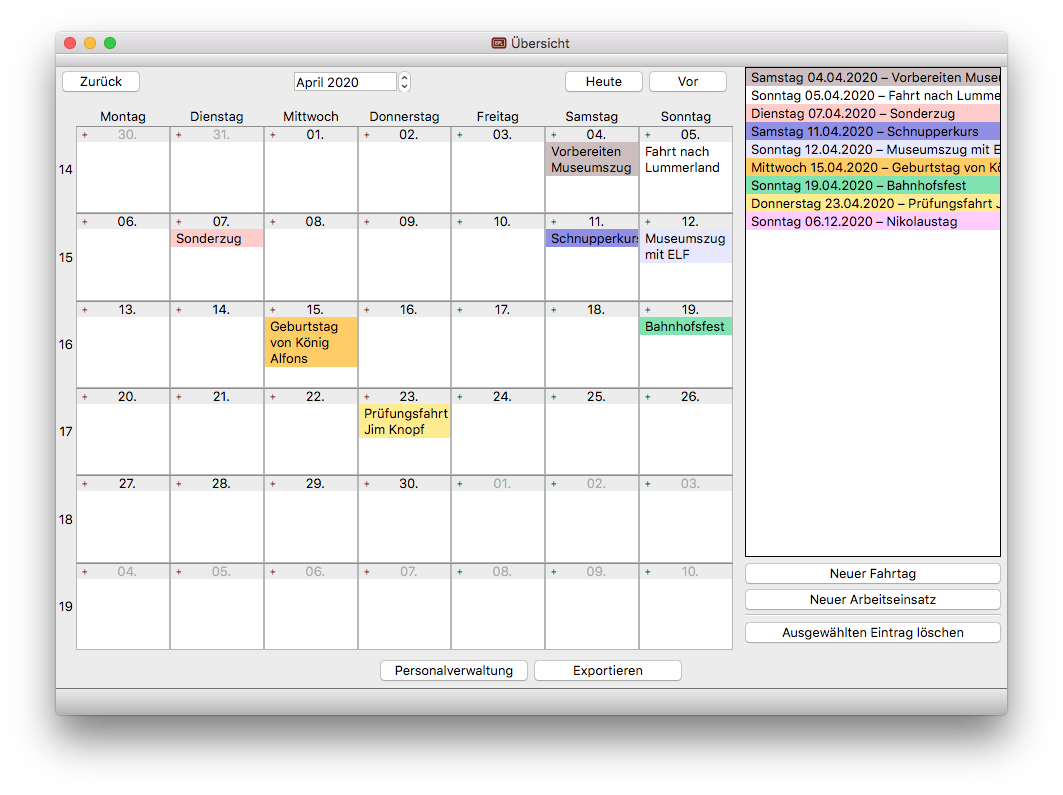
\includegraphics[width=\textwidth]{img/kalender}
  \caption{
  Startfenster des \Einsatz mit dem Kalender und den eingetragenen Fahrtagen und Arbeitseinsätzen}
  \label{fig:einsatz:kalender}
\end{figure}



\section{Aktivitäten verwalten}
\label{einsatz:kalender:anlegen}
\label{einsatz:kalender:löschen}
\paragraph{Fahrtag erstellen}
Um einen neuen Fahrtag anzulegen, klicken Sie auf den Knopf \button{Neuer Fahrtag}.
Es wird ein Fahrtag mit dem aktuellen Datum angelegt und das entsprechende Fenster geöffnet (siehe \cref{einsatz:fahrtag})

\paragraph{Arbeitseinsatz erstellen}
Ein neuer Arbeitseinsatz kann mit Hilfe des Knopfes \button{Neuer Arbeitseinsatz} angelegt werden.
Ein Arbeitseinsatz kann auch direkt im Kalender mit einen Klick auf \button{+} mit dem entsprechenden Datum erstellt werden.
In beiden Fällen öffnet sich danach das Fenster für den Arbeitseinsatz
(siehe \cref{einsatz:arbeitseinsatz}).




\paragraph{Löschen von Aktivitäten}
Um eine Aktivität zu löschen, wählen Sie diese in der Liste aus
und klicken auf den Knopf \button{Listeneintrag löschen}.
Nach einer Sicherheitsabfrage wird der Eintrag gelöscht und verschwindet dann auch aus dem Kalender.



\section{Navigation im Kalender}\label{einsatz:kalender:navigieren}
Mit den Knöpfen \button{Zurück}, \button{Vor} und \button{Heute} können Sie durch den Kalender navigieren.
Ebenso können sie über das Feld auch direkt ein Datum eingeben.



\section{Das Datei-Menü}
Im Datei-Menü stehen Ihnen folgende Funktionen zur Verfügung:
\begin{description}
  \item[Neu]
  Erstellt ein neues Fenster mit einer leeren Einsatzplaner-Instanz.

  \item[Öffnen \dots]
  Es wird ein Dialog geöffnet, mit dem eine \datei{.ako}-Datei geöffnet werden kann.

  \item[Zuletzt benutzt]
  Unter diesem Eintrag finden Sie die fünf zuletzt verwendeten Dateien.
  Sie können direkt geöffnet werden.
  Ebenso können Sie bei Bedarf die Liste leeren.

  \item[Speichern]
  Die Datei wird an dem bisher bekannten Pfad gesichert, oder Sie werden nach einem Ort zum Sichern der Datei gefragt.

  \item[Sichern unter \dots]
  Sie können einen Ort auswählen, an dem die Datei gespeichert werden soll.
  Zur automatischen Speicherung der Daten finden Sie in \cref{epl:allg:einstellungen} weitere Informationen.

  \item[Stammdaten sichern unter \dots]
  Diese Funktion bietet die Möglichkeit, die unveränderlichen Personaldaten zu exportieren.
  Ebenso werden die Datei-Einstellungen übernommen.
  Es werden somit keine Fahrtage oder Arbeitseinsätze gespeichert.
  Diese Funktion dupliziert sozusagen die aktuelle Datei und löscht dabei alle Fahrtage und Arbeitseinsätze.


  \item[Eigenschaften]
  Hier können Sie das Online-Tool aktivieren und konfigurieren.
  Weitere Informationen in \cref{einsatz:kalender:upload}.

  \item[Schließen]
  Schließt das aktuelle Fenster.
  Bei ungesicherten Veränderungen wird vor dem Schließen nachgefragt, ob die Änderungen gespeichert werden sollen.
  Wenn kein Fenster mehr geöffnet ist, wird das Programm beendet.

  \item[Export \dots]
  Ruft die Exportfunktion auf.
  Weitere Funktionen in \cref{einsatz:kalender:export}.
\end{description}


\section{Export}\label{einsatz:kalender:export}
\begin{figure}[!h]
  \centering
	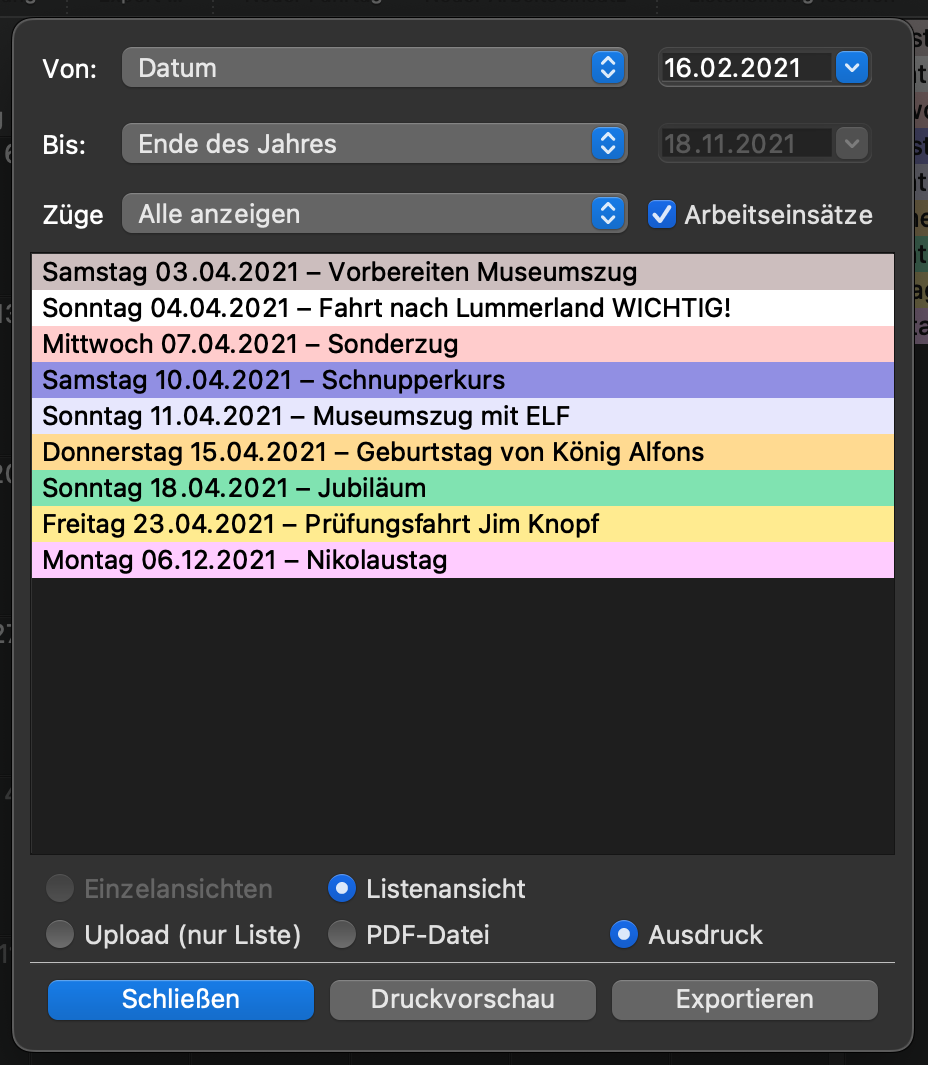
\includegraphics[width=.5\textwidth]{img/export}
	\caption{Der Exportdialog im Hauptfenster.}
	\label{fig:einsatz:kalender:export}
\end{figure}
Über den Knopf \button{Export} öffnet sich der Dialog in \cref{fig:einsatz:kalender:export}.
Diese Funktion ist auch über den Tastaturbefehl \cmnd{cmd+P} beziehungsweise \cmnd{ctrl+P} zu erreichen.

Dort kann mit den beiden Auswahlfeldern am oberen Ende eine zeitliche Beschränkung der Aktivitäten angegeben werden.
Mit dem darunterlegenden Auswahlfeld, kann bestimmt werden, welche Art von Fahrtag exportiert werden soll (z.B.\ nur Nikolauszüge).
Auch kann hier ausgewählt werden, ob die Arbeitseinsätze nicht ausgegeben werden sollen.

Alle Aktivitäten, die in der Liste angezeigt werden, werden bei einem Export per Listenansicht ausgegeben.

Um eine Einzelansicht einzelner Aktivitäten auszugeben, müssen Sie die entsprechenden Aktivitäten in der Liste durch einen Klick auf das Element auswählen bzw.\ abwählen.

Um die entsprechenden Ansichten zu generieren,
wählen Sie das entsprechende Auswahlfeld.
Ebenso können Sie hier bestimmen, ob die Ausgabe als PDF-Datei auf den zuvor konfigurierten Webserver hochgeladen (\cref{einsatz:kalender:upload}),
als PDF-Datei gespeichert oder auf einem Drucker gedruckt werden soll.
Für den Export in eine PDF-Datei wird ein Fenster geöffnet, in dem Sie den Speicherort auswählen können.
Sollten Sie die Dokumente drucken wollen,
öffnet sich das Drucker-Fenster Ihres Betriebssystems,
in dem Sie weitere Einstellungen vornehmen können (Papierformat, Ausrichtung, \dots).
\begin{neu}
Ebenso besteht die Möglichkeit per Knopfdruck eine Druckvorschau anzuzeigen.
Aus dieser heraus kann dann direkt gedruckt werden.
\end{neu}

Die Einzelansicht kann für jede Aktivität auch im entsprechenden Fenster direkt generiert und als PDF gespeichert oder gedruckt werden.




\section{Upload-Tool}\label{einsatz:kalender:upload}
Dieses Tool gibt ihnen die Möglichkeit die Listenansicht des Einsatzplans als PDF-Datei auf einen Webserver hochzuladen.
Dies kann manuell oder automatisch bei jedem Speichern geschehen.
Zur Konfiguration befindet sich im \aktion{Datei}-Menü ein Punkt \aktion{Eigenschaften}.
Durch diesen öffnet sich der Abschnitt in \cref{fig:einsatz:kalender:upload}.
Relevant ist hier der obere Teil.
\begin{figure}[!h]
  \centering
	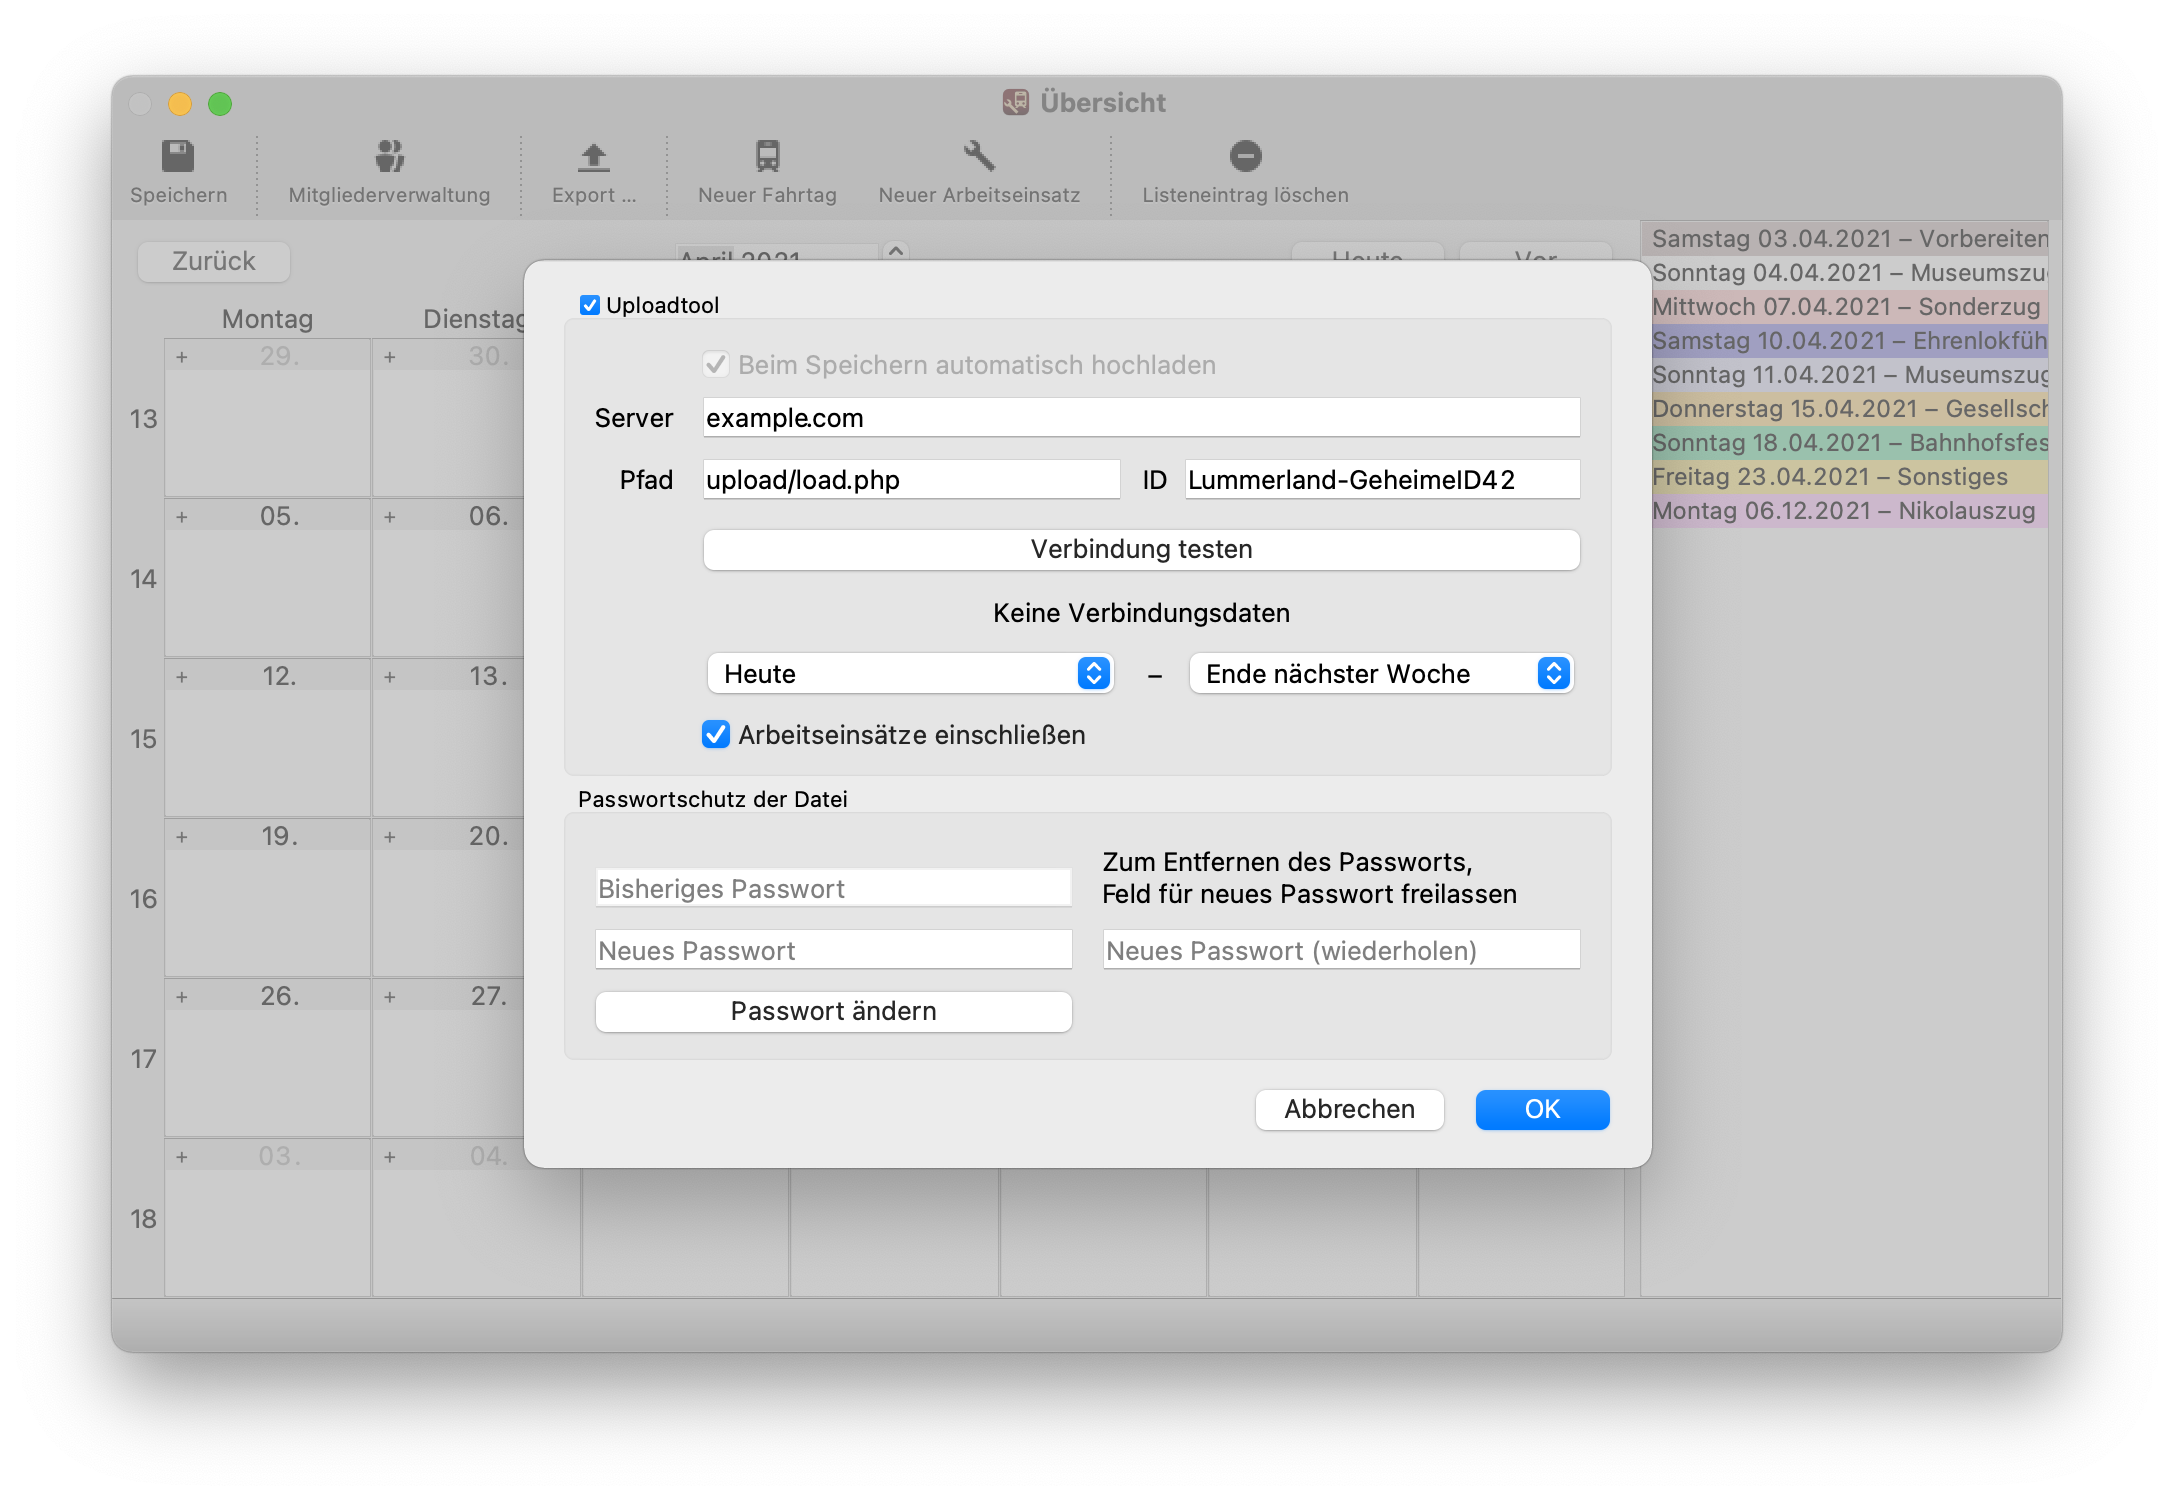
\includegraphics[width=0.5\textwidth]{img/eigenschaften}
	\caption{Des Fenster der Dateieigenschaften}
	\label{fig:einsatz:kalender:upload}
\end{figure}
\begin{itemize}
  \item
  Mit dem ersten Haken wird das Tool aktiviert.
  \item
  Der zweite dient dazu einzustellen, ob die Datei automatisch hochgeladen wird, wenn die lokale Datei gespeichert wird.
  Diese Funktion ist nur verfügbar, wenn sie in den Programmeinstellungen aktiviert wurde (siehe \cref{epl:allg:einstellungen}).
  \item
  Unter Server, Pfad und ID geben Sie die Daten an, die Ihnen von Ihrem Webmaster mitgeteilt wurden.
  Standardmäßig wird HTTPS als Protokoll verwendet.
  \item
  Mit dem Knopf können Sie testen, ob die Eingaben korrekt sind und eine Verbindung zum Server aufgebaut werden kann.
  Dabei werden keine Daten der Aktivitäten übermittelt.
\end{itemize}
Die drei letzten Einstellungen werden benötigt, wenn die Listenansicht automatisch hochgeladen werden soll.
Sie können einstellen, in welchem Zeitraum die Aktivitäten liegen müssen, damit Sie eingeschlossen werden.
Ebenso können Sie auswählen, ob Arbeitseinsätze auch ausgegeben werden sollen.

\begin{hinweis}
  Beim Verwenden der Export-Funktion aus \cref{einsatz:kalender:export} können Sie Beschränkungen festlegen, die unabhängig von diesen Einstellungen sind.
\end{hinweis}

\begin{neu}
\begin{hinweis}
  Bei einer unsicheren Serververbindung (d.h.\ Sie verwenden HTTP als Protokoll und nicht HTTPS),
  wird der automatische Upload aus Sicherheitsgründen deaktiviert.
  Der manuelle Upload bleibt aber weiterhin möglich.
\end{hinweis}
\end{neu}
